\documentclass[tikz,border=5pt]{standalone}
\usetikzlibrary{arrows.meta}
\usetikzlibrary{backgrounds}
\usetikzlibrary{calc}

\usepackage[T1]{fontenc}
\usepackage{lmodern}
\usepackage{mathtools}
\newcommand*{\TickSize}{2pt}%

\begin{document}
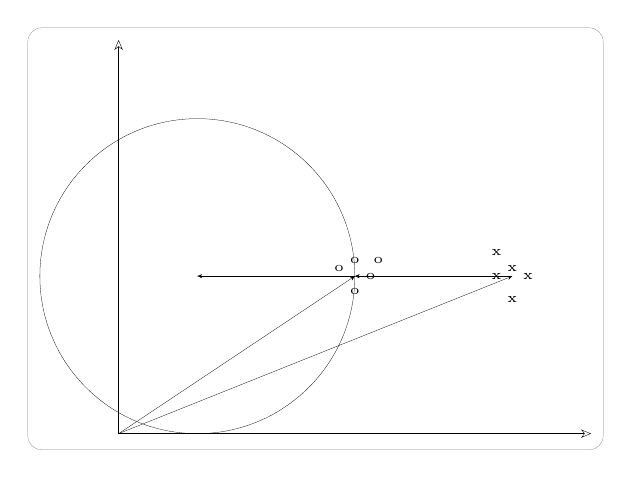
\begin{tikzpicture}
	[framed,background rectangle/.style={ultra thin, rounded corners=5pt, draw=gray}];

	%Axis
	\coordinate (x) at (6,0);
	\coordinate (y) at (0,5);
	\coordinate (o) at (0,0);
	\draw[-{Stealth[scale=1.0,angle'=45,open]}, line width=0.05mm] (o)--(x); %node [midway, below, sloped, align=center]{\tiny Document Length};
	\draw[-{Stealth[scale=1.0,angle'=45,open]}, line width=0.05mm] (o)--(y); %node [midway, above, sloped, align=center] {\tiny Normalizer=$1-b+b\dfrac{|d|}{\textrm{avdl}}$};
	\coordinate (r) at (3,2);
	\coordinate (nr) at (5,2);
	\coordinate (new) at (1,2);

	\draw[-{Stealth[scale=0.5,angle'=45]},ultra thin] (o) -- (r);
	\draw[-{Stealth[scale=0.5,angle'=45]},ultra thin] (o) -- (nr);
	\draw[{Stealth[scale=0.5,angle'=45]}-,ultra thin] (r) -- (nr);
	\draw[-{Stealth[scale=0.5,angle'=45]},ultra thin] (r) -- (new);

	%nr
	\node at (5,2.1) {\tiny x};
	\node at (4.8,2) {\tiny x};
	\node at (5.2,2) {\tiny x};
	\node at (5,1.7) {\tiny x};
	\node at (4.8,2.3) {\tiny x};

	%r
	\node at (3,2.2) {\tiny o};
	\node at (3,1.8) {\tiny o};
	\node at (2.8,2.1) {\tiny o};
	\node at (3.2,2) {\tiny o};
	\node at (3.3,2.2) {\tiny o};

	\draw[ultra thin] (1,2) circle (2 cm);
	%==================================================================================
	%\node at (3.3,0.1) {\tiny avdl};
	%\draw[dotted] (3,0) --(3,1.5);

	%\draw[gray,line width=0.05mm] plot [domain=0:6.5] (\x,{1}) node[anchor=north,font=\fontsize{3.5}{3.5}\selectfont]{$b = 0$} ;
	%\draw[blue,line width=0.05mm] plot [domain=0:6.5] (\x,{1-0.25+0.25*(\x/3)}) node[anchor=south,font=\fontsize{3.5}{3.5}\selectfont]{$b = 0.25$} ;
	%\draw[red] plot [domain=0:6] (\x,{1-0.75+0.75*(\x/3)}) node[anchor=west]{\tiny $b = .75$} ;
	%\draw[red,line width=0.05mm] plot [domain=0:6.5] (\x,{1-1+1*(\x/3)}) node[anchor=south,font=\fontsize{3.5}{3.5}\selectfont]{$b = 1.0$} ;

	%\draw[{Stealth[scale=0.3,angle'=45]}-{Stealth[scale=0.3,angle'=45]}, ultra thin] (4,1) -- (4,1.33);
	%\node[font=\fontsize{2.5}{3.5}\selectfont] at (4.3,1.25) {penalty};
	%\draw[{Stealth[scale=0.3,angle'=45]}-{Stealth[scale=0.3,angle'=45]}, ultra thin] (5.5,1) -- (5.5,1.2);
	%\node[font=\fontsize{2.5}{3.5}\selectfont] at (5.8,1.1) {penalty};

	%\draw[{Stealth[scale=0.3,angle'=45]}-{Stealth[scale=0.3,angle'=45]}, ultra thin] (2,1) -- (2,0.67);
	%\node[font=\fontsize{2.5}{3.5}\selectfont] at (1.8,0.8) {reward};
	%\draw[{Stealth[scale=0.3,angle'=45]}-{Stealth[scale=0.3,angle'=45]}, ultra thin] (0.5,1) -- (0.5,0.79);
	%\node[font=\fontsize{2.5}{3.5}\selectfont] at (0.7,0.93) {reward};
\end{tikzpicture}
\end{document}